% L13b student companion deck: interpretable allocation and model-predictive rebalancing,
% an extended version of the INFORMS Annual Meeting 2026 talk (arXiv:2611.03022).
%
% November 12, 2026. The frame order mirrors the lecture notebook, which follows the talk:
% allocation, rebalancing, market generator. The disclaimer is slide 2, by instructor
% preference. The four figures are the talk's own, built in ../figs from the talk's sources.
% November 13, 2026: trimmed with the notebook. The score frames now come before the
% utility problem, as in the notebook, and the wording follows the trimmed notebook text.
% Notation follows the lecture: score \gamma_i, market state \xi with gain G, market growth
% rate \tilde g_M, basket \mathcal{N} of K stocks, shares n_i, weights w_i, single-name cap
% \bar w, growth-rate covariance \Sigma_g, volatility cap \sigma_SPY, half spread \bar c,
% turnover budget B, beta cap \bar\beta, forecast mean and SD \mu_W(\tau), \sigma_W(\tau).
\documentclass[aspectratio=169,11pt]{beamer}
\usepackage{vnslides}

\newcommand{\Nc}{\mathcal{N}}
\newcommand{\repo}{https://github.com/varnerlab/CHEME-5660-CourseRepository-Fall-2026/blob/main/lectures/week-13/L13b}

\title{\texorpdfstring{{\vnheavy L13b}}{L13b}: Interpretable Allocation and Model-Predictive Rebalancing}
\subtitle{CHEME 5660 Cornell University}
\author{Copyright Jeffrey Varner 2026. All Rights Reserved}

\begin{document}

\vntitlepage

\begin{frame}{Disclaimer and Risks}
  \vspace{0.6em}
  \textbf{\ink{Training only.}} This content is for training and informational
  purposes only. The teaching team does not make, give, or endorse any offer or
  solicitation to buy or sell securities or derivative products, or provide
  investment or trading advice or strategy.

  \vspace{1.1em}
  \textbf{\ink{Risk.}} Trading involves risk and is generally not recommended for
  those with limited resources, experience, or a low risk tolerance. Past
  performance does not guarantee future success.

  \vspace{1.1em}
  \textbf{\ink{Responsibility.}} You are responsible for your investment decisions
  based on your financial circumstances, objectives, risk tolerance, and
  liquidity needs.
\end{frame}

\begin{frame}{Objectives for Today}
  Previously, we chose the share counts of a portfolio once. How do we manage that
  portfolio every day, and how do we judge it when the real market gives us only one path?

  \vspace{0.5em}
  {\large\textbf{\ink{Today's concepts}}}
  \begin{itemize}\setlength{\itemsep}{0.4em}
    \item \hilite{Allocation}: maximum utility within a budget and trading limits, with
      a score for each stock that combines its expected growth rate with the market state.
    \item \hilite{Rebalancing}: a model-predictive controller that re-plans at the
      horizon, at a band exit, or at a drawdown stop.
    \item \hilite{Evaluation}: one historical path, and then typical and stressed
      synthetic markets.
  \end{itemize}
\end{frame}

\begin{frame}{What You Need to Know}
  \vspace{0.3em}
  {\large\textbf{\ink{Core concepts}}}
  \begin{itemize}\setlength{\itemsep}{0.15em}
    \item Each rebalance maximizes a utility of the stock scores within a budget and four
      trading limits. The score has the sign of the stock's expected growth rate, and the
      market state changes only its size.
    \item The method re-plans after 21 trading days, when the wealth leaves the 95\%
      forecast band, or when it falls 8\% below its peak.
    \item A backtest is one historical path. A market generator fitted to the same stocks
      gives many typical and stressed markets for testing the same method.
  \end{itemize}

  \vspace{0.3em}
  {\large\textbf{\ink{For understanding}} \dimmed{(you won't reproduce these)}}
  \begin{itemize}\setlength{\itemsep}{0.2em}
    \item The four utilities, their solutions under the budget alone, and the three benchmarks.
    \item The forecast model, the market hedge, and the trading costs.
    \item The ten selection rules, and how the typical and stress sets are chosen.
  \end{itemize}
\end{frame}

\begin{frame}{Lectures and Examples}
  \vspace{0.3em}
  {\normalsize\textbf{\ink{Lecture:}}\par\small
  \href{\repo/CHEME-5660-L13b-Lecture-MPC-Allocation-Fall-2026.ipynb}{\dimmed{CHEME-5660-L13b-Lecture-MPC-Allocation-Fall-2026.ipynb}}}

  \vspace{0.6em}
  {\normalsize\textbf{\ink{Examples:}}\par\small
  \href{\repo/CHEME-5660-L13b-Example-MPC-RealData-Fall-2026.ipynb}{\dimmed{CHEME-5660-L13b-Example-MPC-RealData-Fall-2026.ipynb}}\par
  \href{\repo/CHEME-5660-L13b-Example-MPC-SyntheticData-Fall-2026.ipynb}{\dimmed{CHEME-5660-L13b-Example-MPC-SyntheticData-Fall-2026.ipynb}}}
\end{frame}

% ========== Live portfolio management
\begin{frame}{Live Portfolio Management}
  \vspace{0.3em}
  Live portfolio management couples three problems: \hilite{allocation} (what to hold),
  \hilite{rebalancing} (when to trade), and \hilite{evaluation} beyond the historical
  record. We'll treat the three problems as one system. We call the portfolio that this
  system manages the \hilite{book}.

  \vspace{0.8em}
  The study uses daily data for 373 S\&P 500 stocks. It calibrates on 2014 to 2024 and
  trades the 420 trading days from January 2025 to September 2026. Every decision uses
  only data available on the day of the decision.

  \slidenote{Study:}{J. D. Varner, INFORMS Annual Meeting 2026, arXiv:2611.03022.}
\end{frame}

% ========== Allocation
\begin{frame}{Allocation: The Score $\gamma$}
  A \hilite{selection rule} picks a basket $\Nc$ of $K$ stocks, or names. A
  \hilite{weighting rule} then chooses the shares $n_{i}\geq 0$ of each stock $i$. The
  method gives each stock a score:
  \begin{equation*}
    \boxed{\gamma_{i}=\tanh\left(\frac{\alpha_{i}+\beta_{i}\,\tilde{g}_{M}}{\max\left(|\beta_{i}|,\,0.1\right)^{\xi}}\right)}
  \end{equation*}
  where $\alpha_{i}$ and $\beta_{i}$ are the single index model parameters of stock $i$
  against \texttt{SPY}. The market growth rate $\tilde{g}_{M}$ is the 252-day EMA of the
  daily growth rate of \texttt{SPY} (units: 1/yr). The numerator is the \hilite{expected
  growth rate}, and the denominator is the \hilite{$\beta$ penalty}.
\end{frame}

\begin{frame}{The Market State}
  The penalty depends on the \hilite{market state} $\xi$, which compares the 21-day and
  the 63-day EMA of the \texttt{SPY} close:
  \vspace{-0.3em}
  \begin{equation*}
    \xi=-G\left(\frac{\text{EMA}_{21}}{\text{EMA}_{63}}-1\right)
  \end{equation*}
  \vspace{-0.3em}
  where the gain $G=21.23$ keeps $|\xi|\leq 1$ on 99\% of the days from 2014 to 2024:
  \begin{center}
    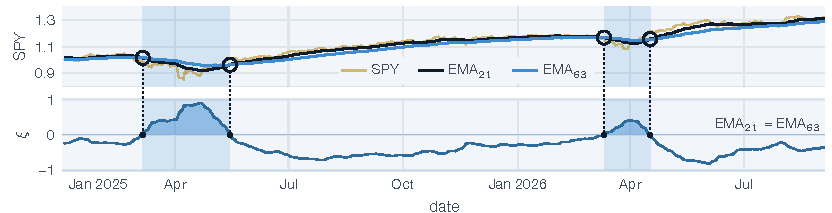
\includegraphics[width=\textwidth,height=0.36\textheight,keepaspectratio]{../figs/Fig-L13b-MarketState.pdf}
  \end{center}
  The top strip shows \texttt{SPY} and its two EMAs, each divided by the first \texttt{SPY}
  close. The market state was positive on the shaded days, 75 of the 420 trading days.
\end{frame}

\begin{frame}{Reading the Score}
  \vspace{0.3em}
  {\large\textbf{\ink{How do we read the score?}}}

  \vspace{0.4em}
  The score has the sign of the expected growth rate, because the $\beta$ penalty is
  always positive.

  \vspace{0.6em}
  In a falling market ($\xi>0$), the penalty shrinks the scores of stocks with
  $|\beta_{i}|>1$ toward zero and favors stocks with a low $\beta$. In a rising market
  ($\xi<0$), the score favors stocks with a high $\beta$.

  \vspace{0.6em}
  The hyperbolic tangent keeps the score between $-1$ and $1$. The absolute value and
  the floor of 0.1 extend the preference weight we used previously to stocks with
  $\beta_{i}\leq 0$.
\end{frame}

\begin{frame}{Maximize Utility Subject to Trading Limits}
  With close price $S_{i}$, wealth $W$, and weight $w_{i}=n_{i}S_{i}/W$, each rebalance
  chooses the shares $n=(n_{1},\dots,n_{K})$ to solve:
  \vspace{-0.3em}
  \begin{equation*}
    \boxed{\begin{aligned}
      \operatorname*{maximize}_{n\,\geq\,0}\quad & U(n;\gamma) &&\quad\text{(utility)}\\
      \text{subject to}\quad & \textstyle\sum_{i\in\Nc}n_{i}S_{i}\leq W &&\quad\text{(budget)}\\
      & w_{i}\leq\bar{w} &&\quad\text{(single-name cap)}\\
      & \sqrt{w^{\top}\Sigma_{g}\,w}\leq\sigma_{\text{SPY}} &&\quad\text{(volatility cap)}\\
      & \bar{c}\,\lVert n-n^{\text{prev}}\rVert_{1}\leq B &&\quad\text{(turnover budget)}\\
      & \beta^{\top}w\leq\bar{\beta} &&\quad\text{(}\beta\text{ cap, hedge on)}
    \end{aligned}}
  \end{equation*}
  where $n^{\text{prev}}$ holds the shares before the rebalance. Wealth that the budget
  leaves unspent stays in cash.
\end{frame}

\begin{frame}{The Trading Limits}
  \vspace{0.2em}
  \begin{center}\small
  \renewcommand{\arraystretch}{1.25}
  \begin{tabular}{@{}>{\raggedright\arraybackslash}p{0.21\textwidth}>{\raggedright\arraybackslash}p{0.40\textwidth}>{\raggedright\arraybackslash}p{0.32\textwidth}@{}}
    \toprule
    \textbf{\ink{Limit}} & \textbf{\ink{What it does}} & \textbf{\ink{Setting in the study}}\\
    \midrule
    Single-name cap $\bar{w}$ & Each stock is at most the fraction $\bar{w}$ of the wealth. &
      $\max(0.10,\,1.5/K)$, which is 11.5\% for 13 stocks\\
    Volatility cap $\sigma_{\text{SPY}}$ & The book is no more volatile than \texttt{SPY},
      where $\Sigma_{g}$ is the covariance of the daily growth rates. & 17.3\% a year\\
    Turnover budget $B$ & A rebalance spends at most $B$ on the half spread $\bar{c}$ per
      share traded. & $0.10\,W$, with a half spread of 5 basis points of the mean close price\\
    $\beta$ cap $\bar{\beta}$ & With the \hilite{market hedge} on, the book's $\beta$ to
      \texttt{SPY} is at most $\bar{\beta}$. & $\max(0,\,1-\xi)$\\
    \bottomrule
  \end{tabular}
  \end{center}
  \vspace{0.3em}
  With the hedge on, the book can also hold up to five stocks with $\beta_{i}\leq 0$.
\end{frame}

\begin{frame}{The Weighting Rules}
  The study compares four utilities of the stocks with $\gamma_{i}>0$:
  \begin{center}\small
  \renewcommand{\arraystretch}{1.35}
  \begin{tabular}{@{}l@{\hspace{2em}}l@{\hspace{2em}}l@{}}
    \toprule
    \textbf{\ink{Utility}} & $U(n;\gamma)$ & \textbf{\ink{Solution with the budget alone}}\\
    \midrule
    Cobb--Douglas & $\sum_{i}\gamma_{i}\ln n_{i}$ & $w_{i}\propto\gamma_{i}$\\
    CES on shares & $\left(\sum_{i}\gamma_{i}\,n_{i}^{\rho}\right)^{1/\rho}$ & $n_{i}\propto\left(\gamma_{i}/S_{i}\right)^{\eta}$\\
    CES on weights & $\left(\sum_{i}\gamma_{i}\,w_{i}^{\rho}\right)^{1/\rho}$ & $w_{i}\propto\gamma_{i}^{\eta}$\\
    Stone--Geary & $\sum_{i}\gamma_{i}\ln\left(n_{i}-b_{i}\right)$ & $\left(n_{i}-b_{i}\right)S_{i}\propto\gamma_{i}$\\
    \bottomrule
  \end{tabular}
  \end{center}
  where $\rho=1-1/\eta$ for the elasticity $\eta=0.5$, and the baseline $b_{i}$ is the number of shares
  worth 1\% of the wealth. With the trading limits, a numerical solver finds the maximum.

  \vspace{0.3em}
  Three benchmarks run under the same limits: minimum variance, the tangency portfolio,
  and a 130/30 long--short book that shorts stocks with $\gamma_{i}<0$. The four utilities
  and the three benchmarks are the seven weighting rules.
\end{frame}

% ========== Rebalancing
\begin{frame}{Rebalancing: The Forecast Band}
  When should the book trade? Trading every day costs money. A fixed calendar ignores
  what the market does between trades.

  \vspace{0.4em}
  The method uses \hilite{model-predictive control}. The controller forecasts the wealth
  of the book and measures the real wealth after each close. When the measurement departs
  from the forecast, the controller makes a new plan, called a \hilite{re-plan}.

  \vspace{0.4em}
  At each re-plan, the controller simulates 1,000 price paths over the next 21 trading
  days with a multi-asset geometric Brownian motion. With $\mu_{W}(\tau)$ and
  $\sigma_{W}(\tau)$ the mean and standard deviation of the forecast wealth $\tau$ trading
  days after the re-plan, the 95\% \hilite{forecast band} is:
  \begin{equation*}
    \mu_{W}(\tau)-1.96\,\sigma_{W}(\tau)\;\leq\;W\;\leq\;\mu_{W}(\tau)+1.96\,\sigma_{W}(\tau)
  \end{equation*}
\end{frame}

\begin{frame}{The Rebalancing Triggers}
  After each close, the controller checks three triggers in order and re-plans on the
  first trigger that holds:
  \begin{enumerate}\setlength{\itemsep}{0.5em}
    \item \hilite{Drawdown stop}: the wealth is more than 8\% below its running peak. The
      re-plan resets the peak to the current wealth.
    \item \hilite{Horizon}: the plan has run for 21 trading days, where the forecast ends.
      The next forecast starts from the measured wealth.
    \item \hilite{Band exit}: the wealth has left the 95\% band. The book has gained or
      lost more than the model expected.
  \end{enumerate}
  \vspace{0.4em}
  Each re-plan solves the same allocation problem from the shares held, with that day's
  estimates. Between re-plans, the book does not trade.
\end{frame}

\begin{frame}{One Episode of the Real-Data Backtest}
  The red line is the wealth of the book divided by its starting wealth $W_{0}$. This book
  holds 13 hand-picked stocks, with the Cobb--Douglas utility and the hedge off:
  \begin{center}
    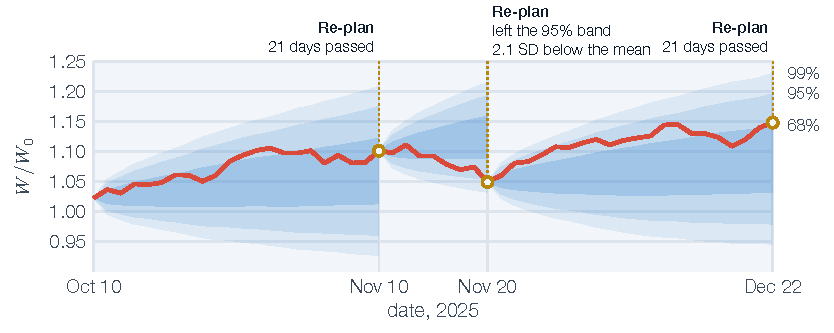
\includegraphics[width=\textwidth,height=0.50\textheight,keepaspectratio]{../figs/Fig-L13b-ForecastBand.pdf}
  \end{center}
  The second re-plan came when the wealth fell 2.1 standard deviations below the forecast
  mean. From January 2025 to September 2026, this book re-planned 27 times: 17 at the
  horizon, 7 at a band exit, and 3 at a drawdown stop.
\end{frame}

\begin{frame}{Fixed Schedule and Trading Costs}
  \vspace{0.3em}
  {\large\textbf{\ink{Do the triggers beat a fixed schedule?}}}

  \vspace{0.3em}
  On a fixed 21-day schedule, the ending wealth was the same. The triggers took about a
  point off the worst drawdown, on real prices and in simulated sell-offs.

  \vspace{1.0em}
  {\large\textbf{\ink{What does a trade cost?}}}

  \vspace{0.3em}
  Each trade fills at the next open and pays a half spread of 5 basis points plus a
  market-impact cost. There is no commission.
\end{frame}

\begin{frame}{The Selection Rules}
  We ran every pair of ten selection rules and seven weighting rules on the real data,
  with the hedge on and off. The selection rules come in three groups:
  \begin{itemize}\setlength{\itemsep}{0.5em}
    \item \hilite{33 stocks, 3 per sector}: in each of the 11 sectors, the rule takes the
      3 highest scores, the top 3 stocks of a bandit, or 3 stocks at random. The bandit
      learns which stocks in a sector grew faster than \texttt{SPY} over the trailing year.
    \item \hilite{13 stocks}: three rules take the 13 highest scores, from the whole
      universe, from the 100 most traded stocks, or skipping a stock correlated above 0.7
      with one already picked. Two random rules draw 13 stocks from the same two pools.
    \item \hilite{Hand-picked}: the book holds 13 stocks chosen by hand without 2025 data
      and never re-picks them. A second list adds WMT and PG.
  \end{itemize}
\end{frame}

\begin{frame}{Selection Matters More Than Weighting}
  Each row is a selection rule, and each dot is a weighting rule:
  \begin{center}
    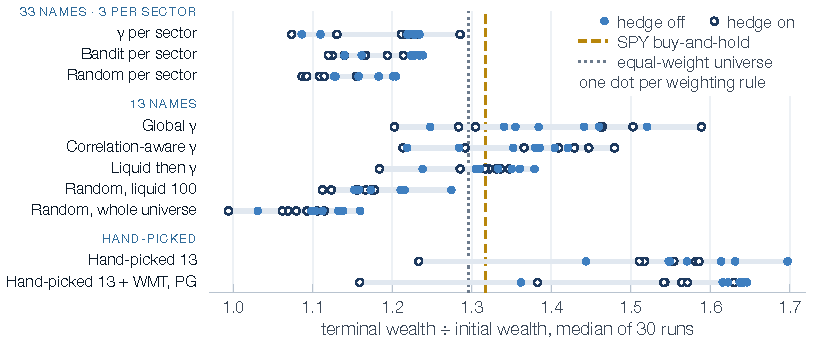
\includegraphics[width=\textwidth,height=0.56\textheight,keepaspectratio]{../figs/Fig-L13b-RealData-Selection.pdf}
  \end{center}
  With the hedge off, seven weighting rules on the 33 stocks picked by score ended between
  1.09 and 1.23 times the initial wealth. Different baskets ended between 1.03 and 1.70.
\end{frame}

\begin{frame}{Example: The Method on Real Data}
  \vspace{0.3em}
  {\normalsize\textbf{\ink{Example:}}\par\small
  \href{\repo/CHEME-5660-L13b-Example-MPC-RealData-Fall-2026.ipynb}{\dimmed{CHEME-5660-L13b-Example-MPC-RealData-Fall-2026.ipynb}}}

  \vspace{0.8em}
  In this example, we run one book day by day. We then change the weighting rule, the
  selection rule, the hedge, and the basket on the same path.

  \vspace{0.8em}
  One path cannot tell us whether a rule was good or lucky.
\end{frame}

% ========== Market generator
\begin{frame}{Market Generator: JumpHMM}
  How do we judge the method beyond the historical record? Real data gives one path of
  prices, with one broad sell-off in the spring of 2025. A market generator gives many
  synthetic markets for the same stocks. The growth rate of synthetic stock $i$ in
  sector $s$ on trading day $t$ is:
  \begin{equation*}
    g_{i}(t)=\underbrace{\alpha_{i}}_{\text{trend}}+\underbrace{\beta_{i}(t)\,g_{m}(t)}_{\text{market}}
    +\underbrace{\delta_{i}\,f_{s}(t)}_{\text{sector}}+\underbrace{\psi_{i}\,\tilde{\varepsilon}_{i}(t)}_{\text{own}}
  \end{equation*}
  where the market, sector, and own draws each come from a jump hidden Markov model
  (JumpHMM). The loadings $\delta_{i}$ and $\psi_{i}$ scale the sector and own draws, and
  each $\beta_{i}(t)$ drifts around the stock's estimate. The generator is fitted to the same 373 stocks on 2014 to 2024. It
  reproduces the fat tails of real growth rates, but its volatility clustering fades
  after a day. The controller still forecasts with a geometric Brownian motion, which
  has no fat tails.
\end{frame}

\begin{frame}{Typical and Stress Sets}
  On each synthetic market, the method calibrates on 2014 to 2024 and trades January
  2025 to September 2026 with the real settings. We draw 10,000 markets and build three
  sets from them:
  \begin{itemize}\setlength{\itemsep}{0.5em}
    \item \hilite{Typical}: this set holds 600 markets drawn at random. The median
      \texttt{SPY} drawdown is 17.6\%.
    \item \hilite{Burst stress}: this set holds the 200 deepest \texttt{SPY} drawdowns
      among markets with a jump burst, months of large moves of both signs. The median
      \texttt{SPY} drawdown is 36.4\%.
    \item \hilite{Bear stress}: this set holds the 200 deepest \texttt{SPY} drawdowns
      among markets without a burst, where prices fall more slowly. The median
      \texttt{SPY} drawdown is 40.6\%.
  \end{itemize}
\end{frame}

\begin{frame}{Sell-Offs: Every Median Ends Above SPY}
  The rows, dots, and lines are as in the real-data figure. Each dot is the median
  across the markets of a set:
  \begin{center}
    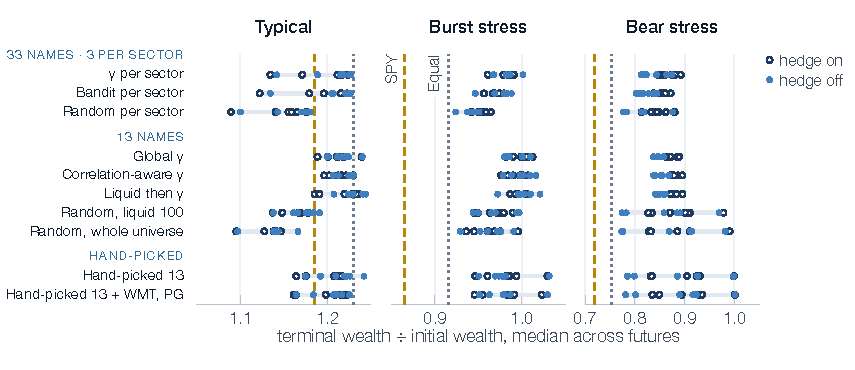
\includegraphics[width=\textwidth,height=0.56\textheight,keepaspectratio]{../figs/Fig-L13b-Synthetic-Sets.pdf}
  \end{center}
  In both stress sets, every median ended above \texttt{SPY} and above the equal-weight
  portfolio. The random selection rules did as well.
\end{frame}

\begin{frame}{Reading the Synthetic Results}
  \begin{itemize}\setlength{\itemsep}{0.7em}
    \item \hilite{The margin}: the margin over \texttt{SPY} came from the allocation, not
      from the timing of the re-plans.
    \item \hilite{Selection by score}: in typical markets with the hedge off, 13 stocks
      picked by score beat 13 random stocks in 62 to 71\% of the markets. In the bear
      stress set, random picks did as well or better for most weighting rules. The
      generator keeps each stock's past trend, which favors selection by score more
      than real prices did.
    \item \hilite{The hedge}: the hedge reduced terminal wealth on real prices, but it
      added to terminal wealth in the bear stress set.
  \end{itemize}
\end{frame}

\begin{frame}{Example: The Method on Synthetic Markets}
  \vspace{0.3em}
  {\normalsize\textbf{\ink{Example:}}\par\small
  \href{\repo/CHEME-5660-L13b-Example-MPC-SyntheticData-Fall-2026.ipynb}{\dimmed{CHEME-5660-L13b-Example-MPC-SyntheticData-Fall-2026.ipynb}}}

  \vspace{0.8em}
  In this example, we run the method on markets from each set and compare the books
  with \texttt{SPY} and an equal-weight portfolio.

  \vspace{0.8em}
  The example uses a few markets in each set, and its counts are rougher than the study's.
\end{frame}

\begin{frame}{Summary}
  \vspace{0.3em}
  We followed one system for managing a stock portfolio every day, from the
  allocation problem to its test on real and synthetic markets.

  \vspace{0.4em}
  {\large\textbf{\ink{Key takeaways}}}
  \begin{itemize}\setlength{\itemsep}{0.4em}
    \item \hilite{In allocation}, stock selection mattered more than the weighting rule.
      Seven weighting rules on one basket ended close together, while different
      baskets ended far apart.
    \item \hilite{In rebalancing}, re-plans came at the horizon, a band exit, or a drawdown
      stop. The triggers gave the same ending wealth as a fixed schedule and took about
      a point off the worst drawdown.
    \item \hilite{In both sell-off sets}, every median ended above \texttt{SPY}. The
      generator keeps each stock's past trend, which favors selection by score.
  \end{itemize}
  \vspace{0.2em}
  A paper-trading version of this system is running now.
\end{frame}

\end{document}
